\section{Refactorings}
\label{sec:refactoring}
After studying thousands of regexes from thousands of Python projects, we have defined a set of equivalence classes for regexes with refactorings that can transform among members in the classes. Figure~\ref{fig:refactoringTree} represents X equivalence classes in grey boxes and various representations of a regex that are all semantically equivalent. The lines between the representations define possible refactorings. The directions of arrows in the possible refactorings will be discussed in Section~\ref{sec:results} based on frequency of occurrence in the community and the understandability of the regexes using 180 study participants. 

Next, we describe each group in detail: 
\paragraph{CCC Group}

\paragraph{DBB Group}

\paragraph{LIT Group}

\paragraph{LWB Group}

\paragraph{SNG Group} This equivalence class contains  three representations of a regex that  deal with repetition of a single element in the regex, represents by \verb!S!. The representation in \emph{S1}, \verb!S{3}!, states that S appears exactly three times in sequence. This can alternately be expressed with a double-bound where the upper and lower bounds are the same, as in \emph{S3}. Removing the repetition symbols in either \emph{S1} or \emph{S3} yields \emph{S2} which is represented explicitly as  \verb!SSS!.  

Using an example from a Python project, the regex\\ \verb!`[^ ]*\.[A-Z]{3}'! is a member of \emph{S1} and could be refactored to \emph{S3} as \verb!`[^ ]*\.[A-Z]{3,3}'!  or to \emph{S2} as \verb!`[^ ]*\.[A-Z][A-Z][A-Z]'!, depending on programmer preferences.





\begin{figure*}[tb]
\centering
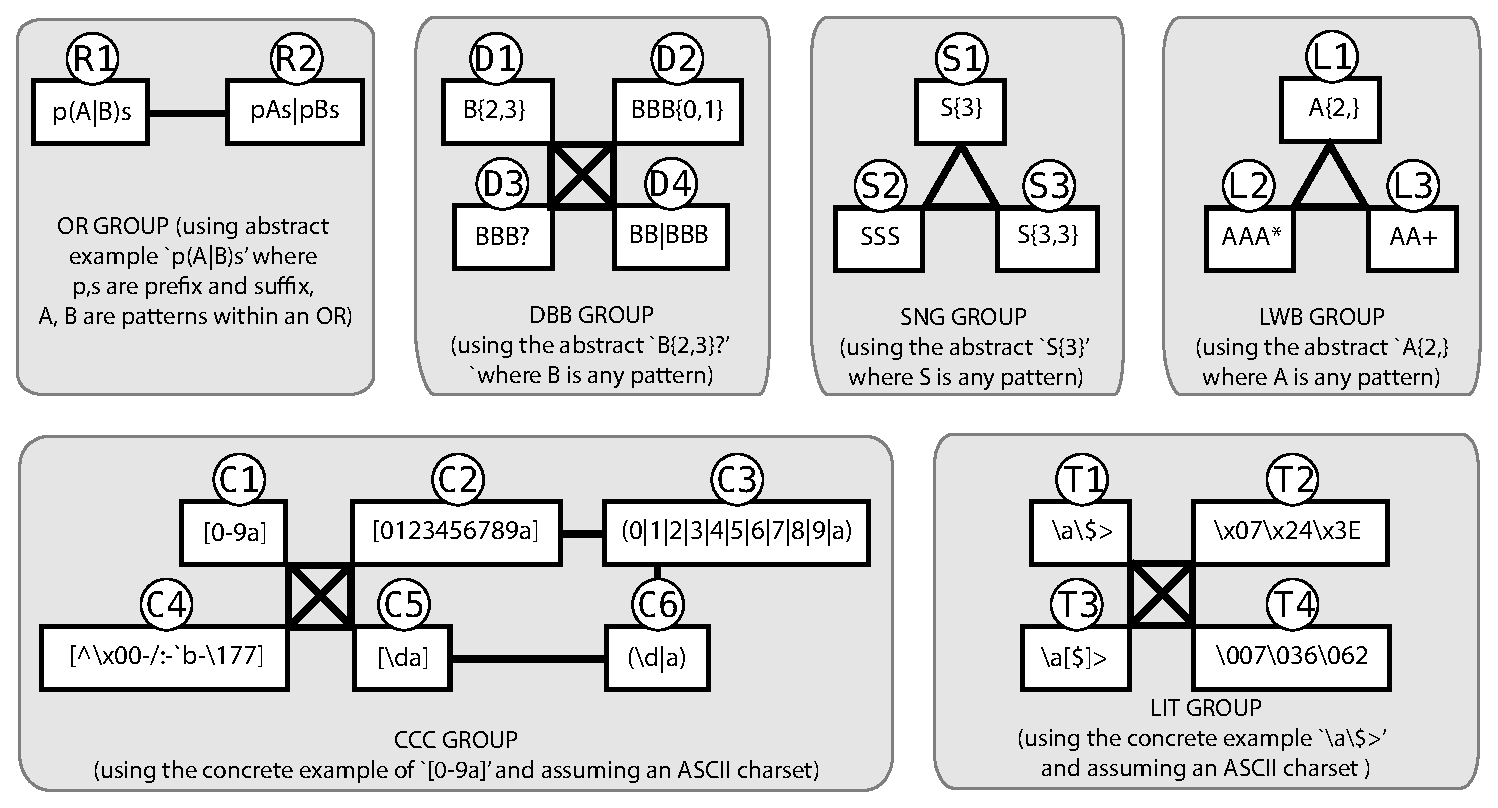
\includegraphics[width=\textwidth]{illustrations/refactoringTree.eps}
\vspace{-12pt}
\caption{Some possible refactorings}
\vspace{-6pt}
\label{fig:refactoringTree}
\end{figure*}















\section{Study}
\label{sec:study}
After defining the possible regex refactorings as described in Section~\ref{sec:refactoring}, we wanted to know which representations in the equivalence classes are considered smelly and which are considered desirable. Desirable for regexes can be defined many ways, including maintainable and understandable. As prior work has shown that regexes are difficult to read~\cite{}, we seek to define refactorings toward understandability. 

We define understandability three ways. First, assuming that common programming practices are more understandable than uncommon practices, we explore the frequencies of each representation from Figure~\ref{fig:refactoringTree} using thousands of regexes scraped from Python projects. Second, we then present people with regexes exemplifying some of the more common characteristics and ask them comprehension questions along two directions: determine which of a list of strings are matched by the regex, and compose a string that is matched by the regex. 

Our overall research questions are:
\begin{description}
\item[RQ1:] Which refactorings have the strongest community support based on how frequently each representation appears in open source Python projects?
\item[RQ2:] Which refactorings have the strongest support based on matching strings?
\item[RQ3:] Which refactorings have the strongest support based on composing strings? 
\item[RQ4:] What is the overlap in the refactoring suggested by RQ1, RQ2, and RQ3? 
\end{description}



First we define a 'Functional Regex'(FR) as some regex that performs in a specific way.  For many FRs, there are several concrete ways to express a single FR.
We define a concrete regex(CR) as a regex expressed with a particular pattern String.
Here is one illustration of these definitions:

\todoNow{create some examples for these terms}

We identified 10 loose groups of FRs, described in this table:

\todoNow{create a table explaining the 10 groups}

For each of these groups we created either two concrete versions of three FRs or three concrete versions of two FRs.

Each of the 10 categories had 6 concrete versions of some FR and so there are 60 CRs.  For each CR, we selected 5 \emph{example strings} designed to test the understanding of the CR.  The idea is that different CRs may have different levels of readability, even when they are representing the same FR.  We define readability as the ability to look at the CR and determine if an \emph{example string} can be matched by it or not.

\todoNow{create some illustration of one matching subtask}


\subsection{Metrics}
We measure understandability of regexes using two complementary metrics, \emph{matching} and \emph{compostition}.

\textbf{Matching:}
 Given a regex and a set of strings, a participant determines which strings will be matched by the regex. The percentage of correct responses is the matching score. For example, consider regex \verb!`RR*'! and five strings, which comes from our study, shown in Table~\ref{matchingmetric}, and the responses from two participants in the \emph{Response 1} and \emph{Response 2} columns. The oracle has the first three strings matching since they each contain at least one \verb!R! character. \emph{Response 1} answers correctly for the first three strings but incorrectly thinks the fourth string matches, so the matching score is $4/5 = 0.80$. \emph{Response 2} misses the second string, so they also scored $4/5 = 0.80$. 


\begin{table}
\caption{Matching metric example \label{matchingmetric}}
\begin{center}
\begin{small}
\begin{tabular} {cl | c c c}
\textbf{String} & \verb!`RR*'! & \textbf{Oracle} & \textbf{Response 1} & \textbf{Response 2} \\ \hline
1 & ``ARROW" 	& \checkmark	& \checkmark	& \checkmark\\
2 & ``qRs" 		& \checkmark	& \checkmark	&\\
3 & ``R0R" 		& \checkmark 	& \checkmark 	& \checkmark\\
4 & ``qrs"		& 			& \checkmark 	&\\
5 & ``98"  		& 			&			&\\ \hline
& Score 		& 1.00		& 0.80		& 0.80 \\
\end{tabular}
\end{small}
\end{center}
\end{table}

\textbf{Composition:}
Given a regex, a participant composes a string that it matches. If the participant is accurate and the string indeed is matched by the regex, then a composition score of 1 is assigned, otherwise 0.  For example, given the regex \verb!`(q4fab|ab)'! from our study, the string, ``xyzq4fab" matches  and would get a score of 1, and the string, ``acb" does not match and would get a score of 0. 

\todoNow{describe how the string was tested against the regex, which libraries, etc.}


\subsection{Design}
In Mechanical Turk, we designed a 180 tasks composed of 10 matching subtasks, so that each of the 60 CRs had 30 separate observations (each an average of 5 \emph{example string} problems).  These 1800 observations are what the analysis will focus on. The ordering of the regexes in each HIT was random to control for learning effects. 


\todoNow{Were there qualification questions that required participants to demonstrate knowledge of regexes?}

\subsection{Participants}
In total, there were 180 different participants in the study. A majority were male (83\%) with an average age of 31. Most had
at least an Associates degree (72\%) and most were at least somewhat familiar with regexes prior to the study (87\%). On average, 
participants compose 67 regexes per year with a range of 0 to 1000. Fittingly, participants read more regexes than they write with an average of 116 and a range from 0 to 2000. Figure~\ref{participantprofile} summarizes the self-reported participant characteristics from the qualification survey. 

Basic regex knowledge test. 4/5 correct to pass. 


\begin{figure}
\fbox{\parbox{\columnwidth}{
\begin{enumerate}
\item 
\begin{tabular} {lrr}
\textbf{What is your gender?} & \textbf{n} & \textbf{\%}\\ \hline
Male & 149 & 83\%\\ 
Female & 27& 15\%\\
Prefer not to say & 4& 2\%
\end{tabular}
\item \textbf{What is your age?} \\
$\mu = 31$, $\sigma = 9.3$

\item 

\begin{tabular} {l |rr}
\textbf{Education Level?} & \textbf{n} & \textbf{\%}\\ \hline
High School & 5 & 3\%\\
Some college, no degree & 46 & 26\%\\
 Associates degree & 14 & 8\%\\
Bachelors degree & 78 & 43\%\\
Graduate degree & 37 & 21\%\\
\end{tabular}
\item 
\begin{tabular} {lrr}
\textbf{Familiarity with regexes?} & \textbf{n} & \textbf{\%}\\ \hline
Not familiar at all & 5 & 3\%\\ 
Somewhat not familiar & 16 & 9\%\\ 
Not sure & 2 & 1\%\\
Somewhat familiar & 121 & 67\%\\
Very familiar & 36 & 20\%\\
\end{tabular}
\item \textbf{How many regexes do you compose each year?} \\
$\mu = 67$, $\sigma = 173$
\item \textbf{How many regexes (not written by you) do you read each year?} \\
$\mu = 116$, $\sigma = 275$
%\item In what contexts do you use regexes? \\
\end{enumerate}
}}
\caption{Participant Profiles, $n=180$ \label{participantprofile}}
\end{figure}